\documentclass{article}

\usepackage[cache=false]{minted}
\usepackage{amsmath}
\usepackage{amssymb}
\usepackage{enumitem}
\usepackage{fontspec}
\usepackage[margin=0.75in]{geometry}
\usepackage{longtable}
\usepackage{booktabs}
\usepackage{graphicx}
\usepackage{wrapfig}
\usepackage{verbatim}

\setmonofont{Fira Code}
\setminted{autogobble}
\usemintedstyle{tango}

\title{Project M -- Report}
\author{Adam Nicholls, George Chichirim, James Hobson, \\ Mihail Denkovski and Minh Le Quoc}

\begin{document}
\maketitle
\begin{quote}
  \textbf{Project M: Put your phone to work}

When people browse social media sites on their phones for hours every day, most of the CPU power goes unused. The old desktop equivalent of this problem was the screen saver, which did little of value until it was co-opted for distributed computing projects such as SETI@home. Your task is to make a platform that can perform useful computation in the background on a large number of mobile phones, while the owners are on social media - or even while they are asleep. It will have to run cross-platform, perhaps using JavaScript, but must also give the appropriate incentives to users - will it drain batteries or incur network charges? If so, what kind of application would customers pay to run on such a platform? Would phone sensors offer any specific value? You need to demonstrate an end-to-end solution including servers, mobile clients and an example application, keeping in mind the security implications if either customers or phone owners try to cheat the system.

[Project in collaboration with G-Research]
\end{quote}
The purpose of this document is to provide documentation, on building and usage of our code, as well as report on how the
code works and our individual contributions, as well as any ethical issues that may arise by the usage of this app.
\tableofcontents
\section{Usage}
The project is split into two parts, the first is the server and the second is the mobile app. Currently there is no way
to build the app for iOS, however a port is in progress so this is subject to change.
\subsection{Building}
The following instructions assume that you are building on a UNIX-Like system and have the following dependencies installed:
\begin{itemize}
  \item{Qt (Tested on version \(\geq 5.12.1\))}
  \item{autoconf}
  \item{Android SDK}
  \item{Android NDK}
  \item{JDK (or openJDK) version \(\geq 8\)}
  \item{GHC}
  \item{Cabal}
\end{itemize}
Autoconf is always needed, the final two dependencies are the server and the rest are for the app. All the additional haskell dependencies are installed
automatically when the \texttt{--enable-autodep} argument is passed to the \texttt{./configure} file.

Build instructions:
\begin{enumerate}
  \item{Clone the git repository \mintinline{bash}{git clone https://github.com/yobson/project-m && cd project-m}}
  \item{Build config files with the \mintinline{bash}{autoconf} command}
  \item{We then configure the program \mintinline{bash}{./configure} command with the following settings:
\begin{longtable}[]{@{}ll@{}}
\toprule
Option & Use\tabularnewline
\midrule
\endhead
\texttt{-\/-disable-app} & Don't build app\tabularnewline
\texttt{-\/-disbale-server} & Don't build server\tabularnewline
\texttt{-\/-enable-autodep} & Automatically install haskell
dependencies\tabularnewline
\texttt{-\/-with-qt-path=\textless{}path\textgreater{}} & Path to Qt
installation. You will probably want to set this\tabularnewline
\texttt{-\/-with-arch=\textless{}arch\textgreater{}} & Set android build
architecture. Options are: arm64\_v8a, armv7, x86\tabularnewline
\texttt{-\/-with-qt-version=\textless{}version\textgreater{}} & Set Qt
version. If not set, will choose newest version installed\tabularnewline
\texttt{-\/-with-live-address=\textless{}web\ address\textgreater{}} &
  Sets server address for app. f unset, will default to the test server \\ & address\tabularnewline
\texttt{-\/-with-projects-list=\textless{}path\textgreater{}} & Set ProjectM
server configuration file path.\tabularnewline
\bottomrule
\end{longtable}
    }
  \item{If all has worked, \mintinline{bash}{make -j} will build the app (\texttt{-j} enables parallel jobs) and produce a 
    file named \texttt{ProjectM.apk} which can be installed on an android phone.}
\end{enumerate}
If for any reason these instructions do not work (or you are trying to build for iOS), open the \texttt{.pro} file in QtCreator.
\newpage
\begin{wrapfigure}[38]{r}{0.5\textwidth}
  \centering
  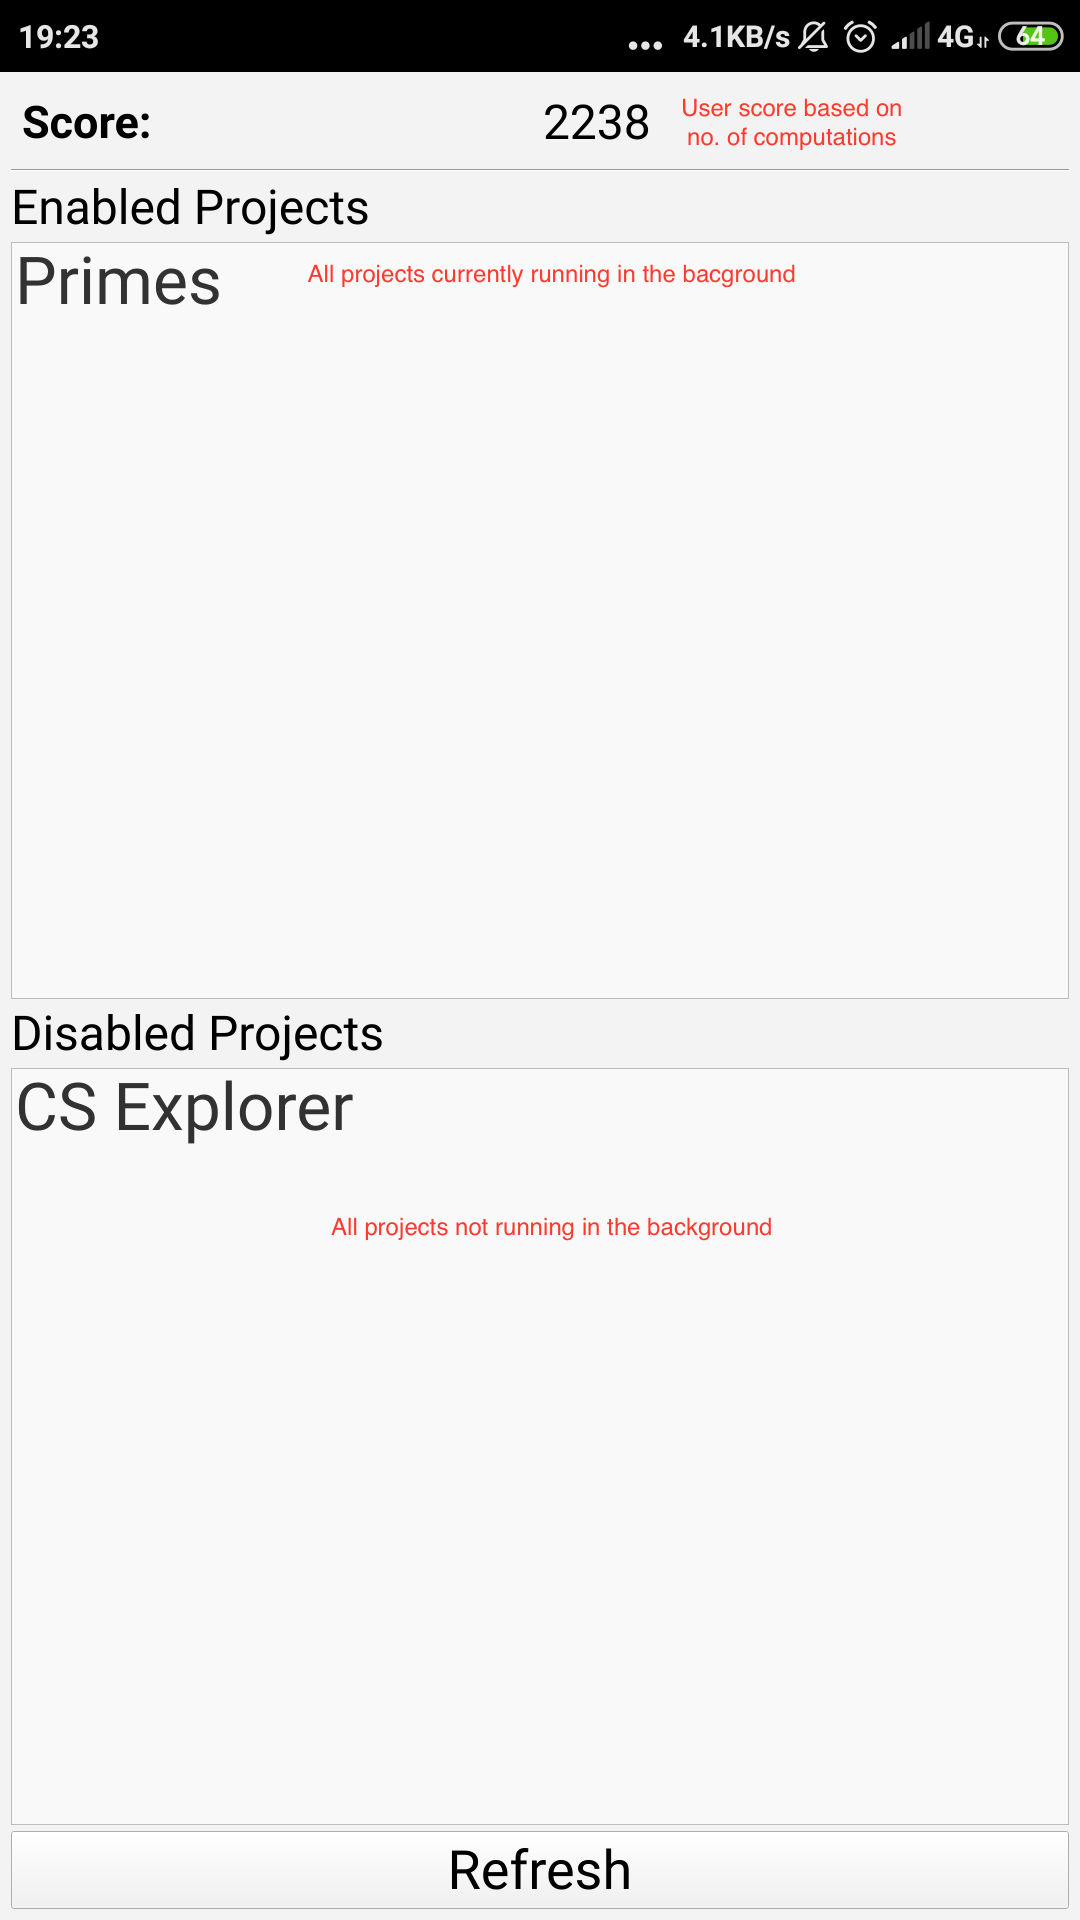
\includegraphics[width=0.5\textwidth]{DocFiles/main_page}
  \caption{Main app page}
\end{wrapfigure}
\subsection{Using the App}
When you launch the app for the first time, you will be prompted for your first and last name. There is no need for a password because
no user data is stored in the server (other than name-id pairs).
When the app is reopened and after registration, the user is greeted with their score and lists of projects. Figure 1 shows 
the main page with the red text explaining what they mean.

Clicking on each project will bring up a new page where you can chose weather to enable or disable each project, decide the 
rate in which the project will run a task (normally between once every 30 second to every 10 minutes). When you enable
a project, if permissions such as location are required, the user will be prompted to choose weather they really want to
enable the project. There is no way that the app can use permissions without the users consent.

\subsection{Configuring the Server}
If you want to host a ProjectM server, their are 3 things you have to consider:
\begin{enumerate}
  \item{Web server software - we use apache for the live server and lighttpt in production but any server with CGI will do e.g. NGINX}
  \item{A place to store the ProjectM Project list - the default is in the tmp directory\dots you really don't want to keep it here!}
  \item{Making sure apps are directed to the right place - the default is \texttt{www.hobson.space}}
\end{enumerate}

Firstly, setting up the server is easy. As long as the \texttt{.cgi} files are in the appropriate place with respect
to your webserver software of choice, for example, in our setup (FreeBSD \& Apache), all of the compiled server files and
projects live in \texttt{/usr/local/www/apache24/cgi-bin/}. It must be the case that all of the \texttt{.cgi} files can be
\textit{accessed} from a web address in the following format `\texttt{base-addr.something/cgi-bin/*.cgi}' Make sure redis is installed!

The ProjectM configuration file is a text file that lists all of the projects in Haskell tuple format.
Here is an example file:
\begin{minted}{haskell}
  ("Project 1", "Description", "project1.cgi")
  ("Project 2", "Description", "project2.cgi")
\end{minted}
You can store this file where ever you like, but you need to specify the location in the configure file with the \texttt{--with-projects-list}

The base address that the mobile app uses is hardcoded for security reasons. This, just like the project list file, also has to specified when building
the app with the \texttt{--with-live-address} option.

\newpage
\subsection{Writing New Projects}
I shall explain how to write a new project with an example.
\begin{minted}{haskell}
import ProjectM

type State = (Integer, Integer, Int) -- Largest, Last Checked, ID of largest

jsMin = "(function(id, number){var n = parseInt(number);"
     ++ "for (var i = 2; i <= Math.sqrt(n); i++)"
     ++ "{if (n % i == 0){return id + \" \" + 0}}"
     ++ "return id + \" \" + n;})"

genPage :: Integer -> Int -> String
genPage prime id = concat ["<head><meta http-equiv=\"refresh\" content=\"30\">",
  "</head><body><h2>Largest prime found is ", show prime, "</h2>",
  "<h3 id=\"finder\">Finder: ", show id,
  "</h3></body>"]

nextOdd :: (Integral i) => i -> i -> i
nextOdd p i | i < p          = p + 2
            | i `mod` 2 == 0 = i + 1
            | otherwise      = i + 2

updater :: Updater State Integer
updater state             RequestJS      = (state, Send jsMin)
updater state@(lg,ch,id)  RequestInput   = ((lg,nextOdd lg ch ,id), 
                                           Send $ show (nextOdd lg ch))
updater state@(lg,ch,id) (ReturnAns n i) | i > lg    = ((i,ch,n), Yeet)
                                         | otherwise = (state, Yeet) 
updater state@(lg,ch,id)  ShowProject    = (state, Send $ genPage lg id)
updater state             RequestPermissions = (state, formatPermissions [])

main = runSite "primes" updater (2,2,1000)
\end{minted}
The general idea is that there is a (user defined) state data type. As the project runs, the project is fed events which
are used to update the state and return input to the phone.
\begin{itemize}
  \item{All ProjectM projects must import \texttt{ProjectM}}
  \item{The \texttt{State} type we define encodes the state at any given point. It must be readable and showable!}
  \item{\texttt{jsMin} is the javascript that is sent to the phone. It is given two string inputs, the first is the user ID and the second is
    a string specified by the server as input (we shall get to that later). This one is a function that checks to see if a number is prime.}
  \item{\texttt{genPage} is an auxiliary function we defined to generate the display page.}
  \item{\texttt{nextOdd} is a function defined to find the next number to check}
  \item{\texttt{updater} is a function that takes a state, event, and returns a tutple, \texttt{(next state, what to return to phone).} You \textbf{must} 
    define this function on all options. The type is \texttt{Updater a b} where \texttt{a} is the state type and \texttt{b} is the type that the phone returns.}
  \item{\texttt{main} function calls \texttt{runSite}. This gets a unique identification string (for DB reasons), the update function and an initial state.}
  \item{This app requires no permissions, but if it did, you would add them to the permissions list (passed to \texttt{formatPermissions}). Currently the only permission
    option is \texttt{Location}.}
\end{itemize}

\section{Project Structure}
The execution of this task is most certainly open to interpretation and fortunately we had the freedom to choose whichever
approach we deemed appropriate given the time restraints. In this section I will outline the general structure of the project as well
as what our aims were when designing. Figure is a UML(ish) diagram showing all of the different parts of our app.
\begin{figure}[h]
  \caption{Diagram describing the structure of the project}
  \centering
  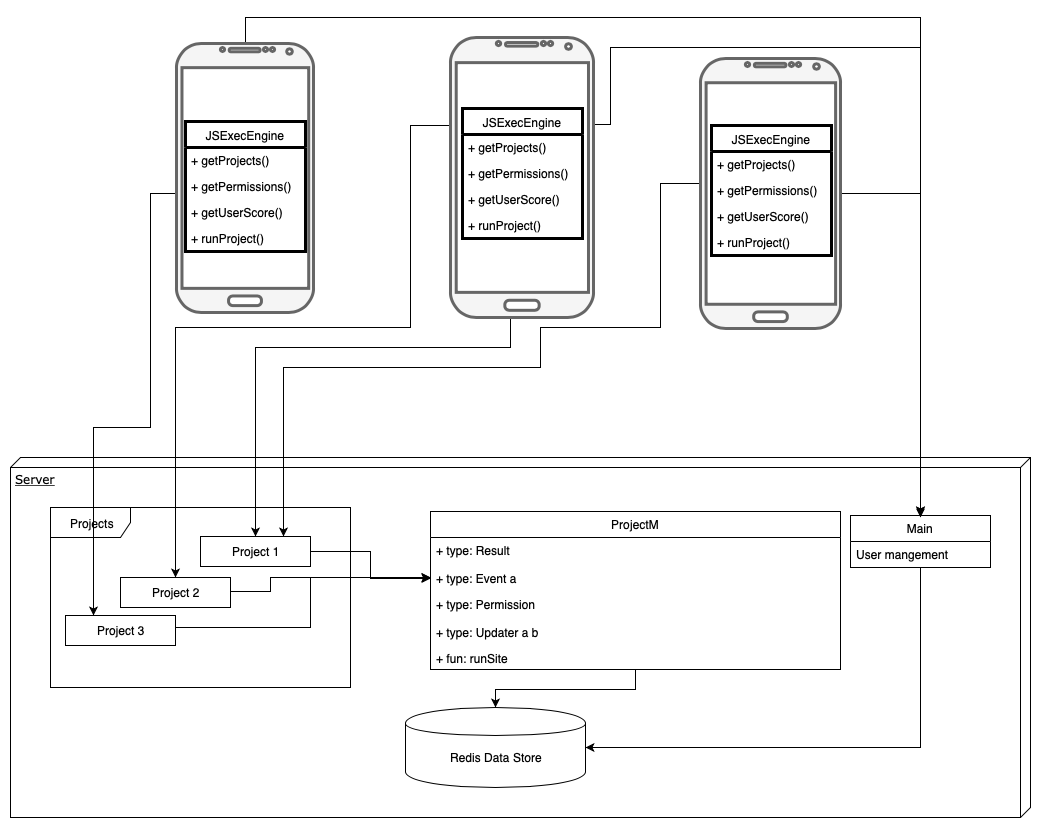
\includegraphics[width=1\textwidth]{DocFiles/ProjectM}
\end{figure}

The server is split into 3 parts: 
\begin{itemize}
  \item{The redis database - not made by us but chosen for high speed and small memory footprint} 
  \item{The main server, used for user management} 
  \item{The projects that make use of the ProjectM library for all access to the phones and resources}
\end{itemize}
All parts of the server are written in Haskell and CGI. Haskell was chosen because it is aggressively type safe and immutability reduces the
chance of obscure runtime errors. As a result, all parts of the server have been running since the first test without a single error! It
was also chosen for the \texttt{ProjectM} library because we wanted to ensure that all of the projects, whoever they are written by,
are up to similar standards of stability. Haskell is a compiled and efficient programming language meaning each project consumed very little space
and many projects can run simultaneously without slowing the server too much. CGI was chosen because we wanted it such that if one app crashed, no others would.
Although there are more modern ways to achieve this, CGI had the advantage of adding negligible size to server binaries and
allows us to add projects and modify existing projects without affecting any of the other projects running.

The mobile app is made up of the following parts:
\begin{itemize}
  \item{Javascript Execution Engine - Deals with all communication between the phone and the server.}
  \item{GUI - The display of the app}
  \item{Background Service - The scheduler and executor of tasks}
\end{itemize}
The app was constructed in C++ using the Qt library. This was chosen because it is cross-platform, allowing us with little additional effort, compile for
every platform. On top of this, with the knowledge that this app was to be running full time in the background of the user's phone, it was crucial to
ensure a little memory and CPU was used as possible, this gives C++ a major advantage over any other cross-platform options as they are almost always
predicated non-native frameworks such as web-technologies or the .net framework.
\section{Detailed Descriptions}
In this section, we shall go into far more detail about how Project M was implemented and tested. We will refer back to the project structure in
many places and so it is suggested that you read that first.
\subsection{Server}
The server is comprised of a user management and project hosting \texttt{CGI} executable and a library that creates project \texttt{CGI} executables.
In order to understand how both work we will need to be fluent in Haskell and know what redis is. Haskell was used for two reasons. The first is that
it is very type safe and has no mutable state making our server code far less prone to errors. The next reason is we wanted the projects to be
programmed in Haskell for the same reason! The two sections (described blow) are in no way linked (other than they share a redis server) and so
could have been programmed in two different languages, but it seemed far more readable to keep all server code in one language.

\subsubsection{User Management and Project Hosting}
The code is found in \texttt{\$PROJECT\_ROOT/Server/main.hs}. Haskell seems like an interesting choice of language for web programming as
the web is aggressively untyped and haskell is aggressively typed, but this was really the reason I decided to use it. All malformed input
must be rejected and all input must be dealt with accurately because this project has the potential to be used in scientific computing!
But for this reason, much of my code involves types of the form \mintinline{haskell}{IO (Maybe a)}. I decided not to use monad transformers
because they seemed not quite up to the job, to instead I defined a nested monadic bind:
\begin{minted}{haskell}
  (|>>=|) :: (Monad m1, Monad m2) => m1 (m2 a) -> (a -> m2 b) -> m1 (m2 b)
  m |>>=| f = fmap (>>= f) m
  infixl 1 |>>=|
\end{minted}
Understanding this code (or at least what it does) will be really useful in Understanding both how the code (and the ProjectM library) work as well as
the policy on malformed input. In essence, it applies monadic bind \textit{within} another monad.

Now we can get onto the two functions of this program. The first is project management. I will not go into much detail about what that means,
for that, read §1.3. The \texttt{getProjects} function is responsible for parsing was is in the configuration file and building
the haskell types. It has to use the strict IO functions in order to guarantee that the file descriptor isn't closed before it has been read.
This would be a problem because we pull the file into a data structure but then close the file and pass that onto another function. Because
haskell is never forced to evaluate the data structure, it never bothers to build it and thus when it is eventually used by \texttt{act},
haskell tries to read the file but it is now closed! This is my justification for the non-standard library usage.

All user function are not concerned with the file system but with the database. The data was chosen to be redis because we really 
valued speed over much else. The library used to interface with redis is `hedis'. Each user function simply runs an hedis query from within the
redis monad, this is then given to us in an \mintinline{haskell}{RedisCtx m f => m (f (Maybe a))} type which take a little refinement to get
back into our preferred \mintinline{haskell}{IO (Maybe a)} type.

Finally, when sending data back to the phone, the standard we decided to use is \texttt{JSON}. For this reason, the type class \texttt{JSON}
has been defined and for every type that is serialized and sent to the phone, there is an instance of the function \texttt{jsonify}.

\subsubsection{ProjectM Library}
The ProjectM library is a library that must be used to create a project that can run on our platform and the code is found at
\texttt{\$PROJECT\_ROOT/Server/ProjectM.hs}. If you have looked at the code (or the code of \texttt{main.hs}) you may have noticed
how much of a mess of monads it is. The idea is that we have messed around with monads so that you, the client, don't have to.

The Library builds \texttt{CGI} programs, not \texttt{FCGI} because we wanted the programs to be easily hot swappable. This means
every single web request to a project launches the program afresh; but there seems to be persistent state in the form of haskell
data types. This is because every single call to the update functions reads the type from the database, changes it and then commits it
back. This gives the illusion that the program is always running. But of course, what if two phone try to change the state at the same time?
This is actually resolved by a certain data structure in redis. The linked list allows us to pop and push objects in linked lists and it blocks
when the list is empty. This is great for us because if we have a singleton list then we can pop the haskell type, blocking all other
processes, then push back on the modified version. This is almost all of what the library does. On top of this, it updates the user's
score whenever they submit an answer, exposes data types needed to implement the user defined functions and provided helpers
and types for permissions.

\subsection{Mobile App}
The app can be be split into a number of distinct parts. The Service is responsible for scheduling runs of the \texttt{JSExecEngine} and is
configured by the GUI. These are the fundamental building blocks of the app.

\subsubsection{Service}
The Service is a background program that needs to schedule runs of the projects according to their own settings and use the \texttt{JSExecEngine} to run them asynchronously. It needs be in perfect coordination with the GUI part where the user can select different configurations for different projects. Unfortunately, every platform handles services differently, and so the Service code needs to be rewritten on every platform. The Android one goes as following:

Firstly, in the \texttt{main.cpp} when the app is started it tries to run the service by the following call:
\begin{minted}{cpp}
QAndroidJniObject::callStaticMethod<void>("space/hobson/ProjectM/MService", "startMService",
        "(Landroid/content/Context;)V", QtAndroid::androidActivity().object());
\end{minted}

\begin{wrapfigure}[12]{R}{0.4\textwidth}
  \centering
  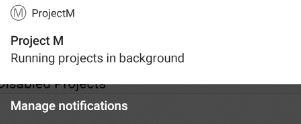
\includegraphics[width=0.4\textwidth]{DocFiles/notification.png}
  \caption{Notification bar}
\end{wrapfigure}

The \texttt{QAndroidJniObject::callStaticMethod} is a function that allows you to call Java functions. It takes the class path, the method name that we want to call, its signature, and the arguments for this method. Here we call the function \texttt{startMService} from the \texttt{MService} class, passing it the current activity. This method is implemented in Java and once called will start the Java Service and will display a notification that lets the user know that projects are running in the background. This service must keep running even though the app is killed.

The C++ implementation of the Service can be found in \texttt{service.h} and \texttt{service.cpp}. There are also \texttt{projectsettings.h} and \texttt{projectsettings.cpp} that contain a lot of constants which will help us to write and read the project settings here and in GUI much easier. The Service works as follow: it triggers every \texttt{ProjectSettings::CHECKING\_FREQ} milliseconds and checks for projects to run. We chose this design because the project settings are quite complex (e.g. Plugged In only or WiFi only) and they can be changed anytime, so this would make the individual scheduling of projects quite impossible. We decided that checking all projects every \texttt{ProjectSettings::CHECKING\_FREQ} milliseconds is the best way.

The project settings are stored using the Qt's \texttt{QSettings} and the constants from \texttt{projectsettings.h}. Apart of these settings which are shared between the Service and the GUI, the Service keeps track of another \texttt{QSettings} file that stores the last times every project was run. There is also a Hash Table \texttt{projectEngines} that keeps track of pointers to instantiated \texttt{JSExecEngine} objects corresponding to the projects.

When the Service is triggered, it goes through every project from the settings file and calls the following function:

\begin{minted}{cpp}
bool shouldRun(QSettings &project, QSettings &lastRun, QString &projectName)
\end{minted}

This will determine if the project should be run now by analyzing all the settings of this project. Here we need to write Java functions that will offer information about the phone:

\begin{minted}{java}
public static boolean isWiFiConnected(Context context)
public static boolean isCharging(Context context)
public static int batteryLevel(Context context)
\end{minted}

And again use the \texttt{QAndroidJniObject::callStaticMethod} to call these methods. If the \texttt{shouldRun} decides that this project should be run then we call the following function that will use the corresponding \texttt{JSExecEngine} object to run the project asynchronously:

\begin{minted}{cpp}
void Service::runProject(QString &projectName, QSettings &settings)
\end{minted}

All through development the Service was continuously tested with sample test data made of all combinations of settings, and since its finalization with live data.

\subsubsection{Java Script Execution Engine}
The Java Script execution engine (found in \texttt{jsexecengine.cpp} and \texttt{jsexecengine.h}) is a class designed to be the bridge between
the server and the rest of the app. It's job is to deal with all server communication as well as executing the JS code on the phone.
I will begin by describing how the object is instantiated and used. The object is instantiated with the following:
\begin{minted}{cpp}
  JSExecEngine *engine = new JSExecEngine(baseAddress, projectExt, parent, editor);
\end{minted}
The \texttt{baseAddress} is the only necessary parameter; the rest have defaults. The base address is the server address such that
\texttt{baseAddress/bin-cgi/} is the directory with the projects and main server app in. The project extension is the name of the
\texttt{cgi} executable (with \texttt{.cgi} extension) of the project it is concerned with (for example \texttt{Primes.cgi}).
The parent is the \texttt{QObject} parent, although not necessary, it does mean that there is elementary garbage collection if
it is instantiated in a tree of \texttt{QObjects}. This is more of a precaution than a necessity, a \texttt{JSExecEngine} object
should be deleted whenever it is done with. The \texttt{editor} is another optional parameter used only in the \texttt{testpage}
class which allows for all logs to be redirected to the screen for testing purposes.

The object is then used using queries and dynamically dispatched callbacks. Luckily, the dynamic callbacks are implemented as part
of the Qt framework. The following queries are available (implemented as public functions):
\begin{minted}{cpp}
void exists_user(QString userID); //Check to see if user exists with certain ID
void register_user(QString firstName, QString lastName); //Register a new user
void get_projects(); //Get list of available projects to run.
void run_project(); //run the selected project (selected when instantiated with projectExt)
void get_score(); //Get user's score
void get_permissions(); //Get permissions needed by selected project
\end{minted}
Notice that every method returns \mintinline{cpp}{void}. This is because the class is designed to be non-blocking and asynchronous.
the following \textit{signals} are also exposed by the class:
\begin{minted}{cpp}
void exists_user_result(bool);
void get_score_result(int);
void register_user_result(QString);
void get_projects_result(QLinkedList<Project>);
void web_error(QNetworkReply::NetworkError);
void get_permissions_result(QStringList permissionList);
\end{minted}
These pretty much correspond to the queries defined above. The following example shows how to use the class to get the user's score:
\begin{minted}{cpp}
void ThisClass::some_func() {
    JSExecEngine *engine = new JSExecEngine(PROJECT_BASE_IP);
    connect(engine, &JSExecEngine::get_score_result, this, &ThisClass::score_slot);
    engine->get_score();
}

void ThisClass::score_slot(int score) {
    //do something with user score
}
\end{minted}

The implementation of theses queries involved a bunch of methods to construct web requests. A struct of type \texttt{nethub\_poll}
is created and filled with data depending on the type of request and response is required. \texttt{enum}s are used to specify
the type of request (corresponding the possible requests to the server) and responses (corresponding to all possible callbacks
both internal and external). The options are:
\begin{minted}{cpp}
  enum query_type {getUser, regUser, noQuery, getProjs, getJS, getJSInput, 
                   returnJS, getPermissions};
  enum return_signal {existsUser, userReg, noSignal, retProjs, jsReady,
                      jsInputReady, retScore, retPermissions, prepPermissions};
\end{minted}
The \texttt{query\_type} is used by a function \texttt{buildRequest} to craft the corresponding GET request. The
\texttt{return\_signal} specifies the return signal and also is used by the \texttt{parseReturn} function to instruct it
how to deal with the data returned by the server. Often queries are made up of many `sequential' web requests. This is dealt with
by chaining internal queries with internal callbacks using the same connection method demonstrated in the get score example.

I am not going to go into too much detail in how this class was constructed, just the core implementation details because it seems
as though every single part of the implementation has some kind of nuance. But I will finish by demonstrating the security and permissions
mechanism:
\begin{minted}{cpp}
            QJSEngine engine;
            QJSValue loc; Coordinate *coord = nullptr;
            if (locationRunning) {
                logger << "Enabling location for:" += baseURL;
                coord = new Coordinate(locationSource->lastKnownPosition().coordinate());
                loc = engine.newQObject(coord);
                engine.globalObject().setProperty("m_location", loc);
            }
            QJSValue fun = engine.evaluate(*instr->data.js);
            QJSValueList args;
            args << *instr->userID << in;
            QJSValue ret = fun.call(args);
\end{minted}
This is the code that runs the JS code on the phone. Notice the \texttt{locationRunning} boolean has to be set in order for the
GPS coordinates to be instantiated. The instantiation of the GPS object is also predicated on that variable, which can only be activated
when the user accepts the permissions. This is low level enforcement of the permission system.

\subsubsection{Graphical User Interface}
The Graphical User Interface was written in C++ using the Qt framework. It consist of two main screens:

The main screen consists of two ListViews representing the enabled and disabled projects, the user score and a refresh button. The ListViews are used with the model-view-controller pattern. This is done by passing the data to a model which provides it to the view:
\begin{minted}{cpp}
    project_list_model_en->setStringList(*project_name_list);
    ui->proj_list_view_en->setModel(project_list_model);    
\end{minted}
The clicks are handled by slots which are normal C++ functions connected to an object and await a particular signal. In this case, upon receiving a click, the project name is extracted and the details are opened in a new ProjectWindow. The ProjectWindow is populated with data passed to its initiallizer.

Data for the ListViews as well as the score is handled by signals and slots which are a central feature of Qt. Signals are emitted when an object is changed in a way which might require an UI change. Slots are then activated by an appropriate signal and handle the received data.

Projects are represented by an object class written using latest C++ guidelines and style. In particular,
classes are encapsulated, the properties are split between public and private and the definition and implementation is split between .h and .cpp files. Class functions are defined using autos and lambdas which improve code clarity. Getters and setters are not the natural paradigm in C++. Instead, properties which are supposed to only have a getter, i.e. are read-only would have a "getter" of the following type:
\begin{minted}{cpp}
    auto name() -> const QString&;
\end{minted}
While properties which are meant to have both getters and setters would have the following:
\begin{minted}{cpp}
    auto enabled() -> bool&;
\end{minted}
which returns a reference through which the value can be read and written. 
\subsection{Testing}
Testing the application was hard given that the specification of each project is up to the creator of the project itself. Having said this,
we have done our best to test our app in a few ways. The first way is by using the app. We have been running the app for (as of writing)
4 weeks. 5 phones minimum have been participating in the Primes project alone and have each been running projects every 30 seconds.
This works out to be almost 100,000,000 exchanges between the mobile app and the server, most of which have been simultaneous. The results
of both test projects have been monitored extensively and there has never been an incorrect result.

We realised that waiting for a bug is not the way to go so have also created a test suit. Launching the app with certain command line
arguments will open onto a page which connects to a different, local, test server and runs stress and accuracy tests in quick succession.
If you want to try this out for yourself, head to the \texttt{tests} branch.

Each part of the UI has been tested by users trying to break it and the service has been tested extensively to make sure that if the user
changes any predicate or changes whether a project is enabled or disabled, the background service will respect the users requests immediately.

\section{Current State of the Project and Possible Future Improvements}
The app is fully functional on android and partially functional on other platforms. The app is built using the Qt framework meaning that
the UI and backend are fully functional on almost all platforms (Windows, Linux, Mac OS, Android, iOS, Blackberry OS, etc.) but
Qt offers no help in developing the background service and this is radically different on every platform. We have only concerned ourselves
with android as it is a platform that we all have access to. Having said that, we have tested all other parts of the app on
Mac OS, Linux and iOS.
\begin{figure}[h]
  \centering
  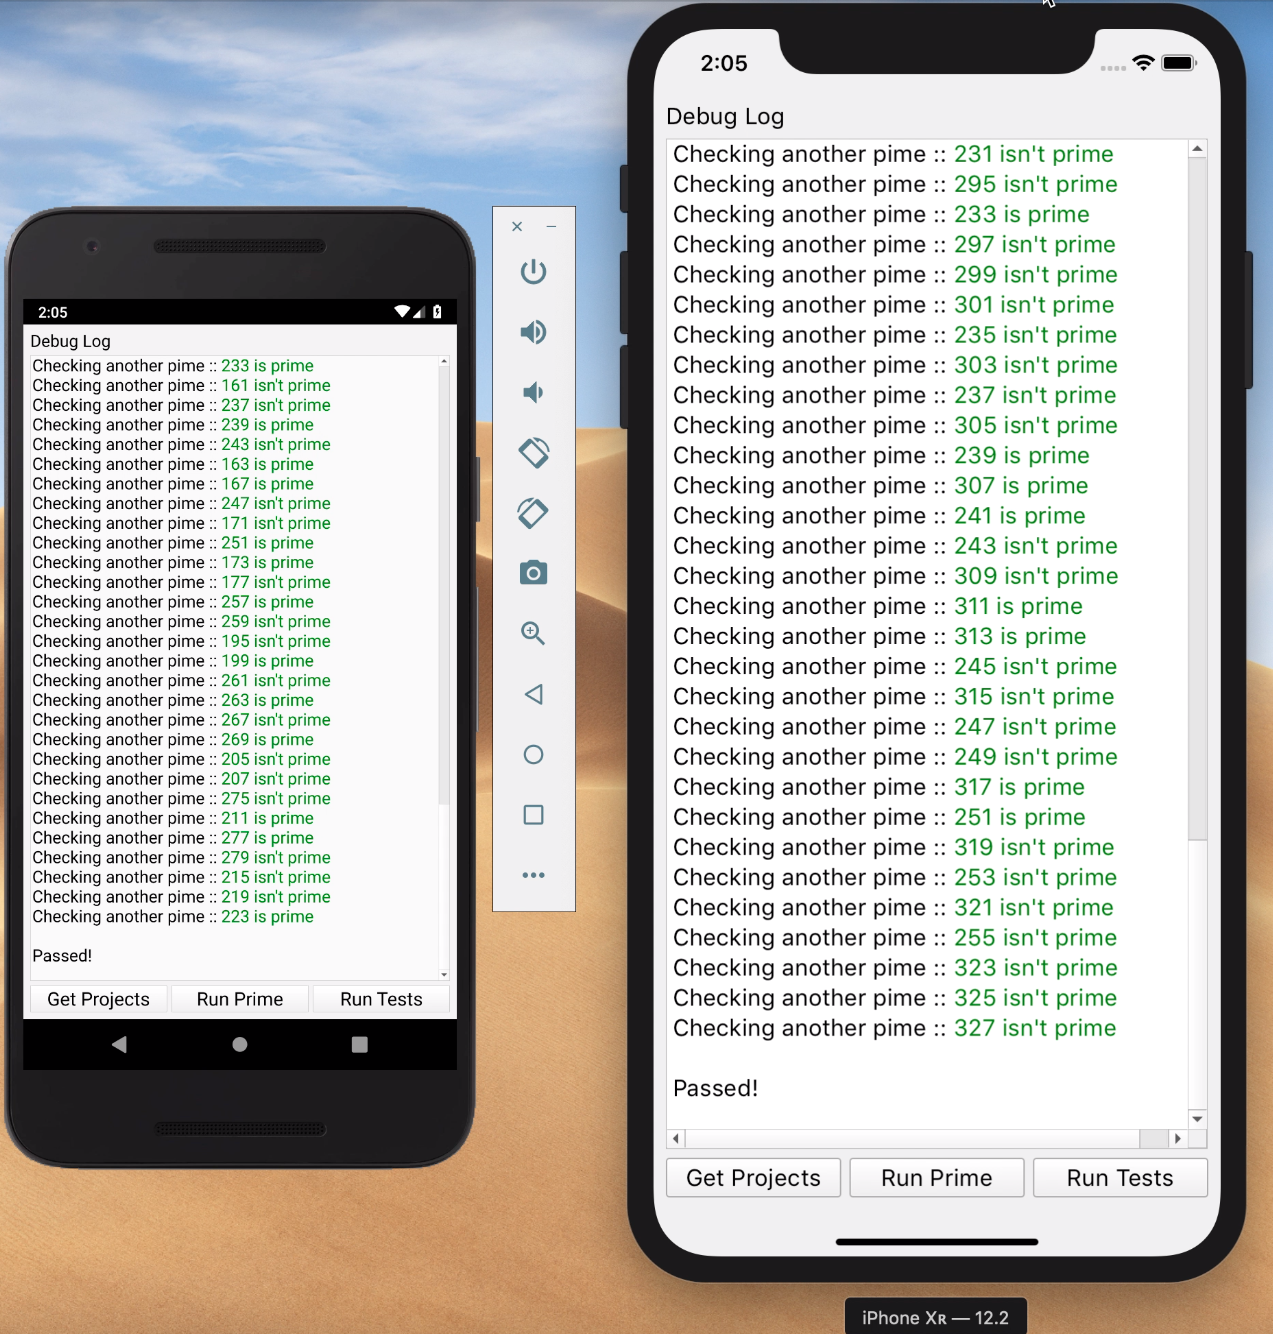
\includegraphics[width=0.5\textwidth]{DocFiles/tests}
  \caption{Automated backend tests running on both Android and iOS}
\end{figure}
If we had more time to develop this project, we would achieve done the following:
\begin{enumerate}
  \item{Remade the UI in QML to achieve a far more user friendly experience while still remaining cross platform}
  \item{Write cross platform service code, although this seems impossible, projects such as GNUstep compile to Mac OS and iOS natively (using Cocoa),
    Windows, Linux and BSD platforms. This would cover all non-mobile targets + iOS}
  \item{Add more sensors and corresponding permissions}
  \item{Write more unit test frameworks for the application}
  \item{Research more how we could incentives people to adopt it}
\end{enumerate}

\section{Responsible innovation}
The system we have created has a range of ethical implications and societal effects that must be considered. We shall also outline possible
security issues and how we have attempted to mitigate them.
\subsection{Ethical Implications}
We should consider what projects we allow users to contribute to through our app. It may be unethical for us to, for example, allow our
users to work on projects that directly contribute to the manufacture, distribution, or use of unethical products such as arms or tobacco.
We must also ensure that users are fully aware of what a particular project is working towards. We should not allow a situation where a project
may seem harmless (given a very limited description) but is really part of a wider project which users may not necessarily want to contribute to.
Furthermore, a project that we allow users to contribute to may be completely benign, but if it is being carried out by a company that employs
unethical practices elsewhere in its business, then we must consider whether we wish to support them by allowing their project on our platform.
This is linked to §5.2.
However, if we decide that we can determine what projects we offer and ban ones we disagree with from our service, one might consider this to mean
that we actively support all projects we are offering and oppose all projects that we remove. This could lead to further issues if we have the
option of hosting or banning projects linked to controversial issues.

Our platform allows us to share sensor data from the user’s phone, and so this puts us in a position of responsibility. We should ensure that
users are aware of exactly what their phone is doing and what they are contributing to when they choose projects to enable. This includes what,
if any, data a project gathers from their phone and what it is used for. Furthermore, we should be able to guarantee to the user that our app
does carry out exactly what the user is expecting it to. For example, a software bug may cause a user’s phone to be contributing to a project
when it appears to be disabled to the user, and this would be a breach of trust, particularly if the user’s phone is mistakenly contributing
to a project that they do not want to support.

An example of a project that is aimed to highlight possible issues with user permission misuse can be found at 
\texttt{http://www.hobson.space/cgi-bin/Explorer.cgi?event=ShowProject}

We have attempted to mitigate some of these issues by building a low level permissions system (more on this in §5.3) meaning that a user can
know exactly what is required from the phone in terms of sensor data. Projects have to be hosted on the same computer as the main server
allowing us to decide which projects can and cannot be run on phones. Although this still suffers from the endorsement issue highlighted in
the second paragraph, we could allow all projects that fit our ethical code and explicitly state that we endorse none of them.

\subsection{Social Effects}
We hope that, if our platform were to be released and widely used, that it could bring awareness and computational resources to many positive
projects and causes. We would be proud to have our platform support any project that aims to make a positive impact in the world, and to have
a userbase that wishes to make a contribution in the form of donating their phones’ spare processing power. However, as mentioned in
§5.1, we must be careful that our platform does not host or support projects that may serve a negative or harmful purpose, whether directly or
indirectly.

Whether our project could be used to bring about positive change is dependent upon what projects become available, but examples of projects
that could be implemented (with arguable efficiency) include protein folding simulations (to aid cancer research), pulsar star analysis
(to aid astrophysical research) and green energy load analysis (to make sure green energy sources are used whenever they can be).

A possible downside of the app is that it may use more energy to solve these problems, but we argue that this is a non-issue. The app was
written in C++ and after 4 weeks of continue testing with the primes experiment, it has consumed 0.7\% of our battery (average). This is
negligible with respect to other apps on the phone. Super computing centres require huge amounts of cooling and energy. There is also the
problem that not many super computing centres run these projects (if any) because the costs are too high and profits non-existent.

\subsection{Data Security}
We have made a number of security considerations when making this app:
\begin{enumerate}
  \item{Internal permissions}
	\item{Low level security}
  \item{User data policy}
  \item{Use of Javascript}
\end{enumerate}
Internal permissions is the idea that default android permissions system is not fine grained enough. The app can request location and sensor
permissions, but really we want each project to request permissions so that the user can have more control over the permission requirements of
each project individually.

This is then implemented with our low level security policy. The Javascript can only be exposed to a certain type of C++ object.
If the permission is not consented by the user, the object relating to the sensor in question is never allocated memory. This way
there is no way, even in the unlikely chance of a remote code execution vulnerability scenario, that an attack could access any data
the user hasn't consented to. This is no help, however, if the user had consented to certain types of data. But we believe that most projects
will not require sensor data meaning that though an attack is theoretically possible, in practice, it would be very hard.

This low level permissions system means that if a project decided to need another permission and doesn't alert the users, the JS will break
because it will require data that is unallocated on the phone.

Another, very simple, approach to data security of users that we have taken is to store almost no data about each user. The data stored is
a name, id and score. The name may as well be fake and duplicates are allowed; it isn't integral to the functioning of the app that this data
be present or correct. We have no intention to store any more user data than this meaning  that in the unlikely event of a security breach,
nothing private would be lost.

When we say that we use javascript, we are not telling the full truth. We are using the full syntax of the language bit a very small
subset of the default functions. This is intentional! There is no way to access any files, make web requests etc so that there is
no way of crafting malicious JS. Any functionality over and above maths (such as accessing location) has to be requested and is implemented
by us so that there cannot be any undefined behaviour.

\section{Group Member Contributions}
\subsection{Adam Nicholls}
As a member of the UI team, I was responsible for using Qt Creator to contribute to the development of a mobile app that will allow a user to
run projects offered by the server. I spent a significant amount of time on some preliminary work that involved setting up Qt Creator and the
Android emulator, familiarising myself with Qt, C++, and git, and gaining a working understanding of the existing code that other group members
had written. I then was able to enhance functionality of the app in a number of ways.

My first responsibility was to find a way for the app to remember the settings that a user selected for each individual project after leaving
the project interface or closing the app altogether. I found that this could be done using Qt’s QSettings class. I thoroughly read up on the
class, what it can do, and the best way to implement it. I then went on to make the necessary changes to projectwindow.cpp to allow the app
to store and recall user settings.

The main window (where available projects are listed) in the first iteration of our app simply contained a single list of all projects that
were returned by the server, with the option to press one to be taken to its specific project settings page. I was tasked with making changes
to this page that allowed the user to more easily see what projects they currently are and aren't contributing to. I researched and experimented
with several different approaches and decided to have the app display two separate lists - one for enabled projects and one for disabled ones.
I was able to implement this by making the required changes to mainwindow.ui and mainwindow.cpp.

In order to control how often a user’s phone contributes to a project, the project settings page contains a slider UI element that lets the user
to select project frequency. I was able to make changes to the app that allowed this construct to be different for each project, rather than
every project being forced to have frequency options of 30, 60, 120, and 300 seconds. To do this, I added to the Project class constructor
\texttt{freq\_values} and \texttt{freq\_labels} parameters, which associate slider positions with a frequency value (in seconds) and a label
to display to the user.

\subsection{George Chichirim}
\subsection{James Hobson}
I was team manager and in charge of the server and parts of the app that interfaced with the server. Although I was manger, a priority of mine
was to ensure that everyone had a say in the design of the app; although as the member with most experience in industry, I decided which tools
and frameworks (such as Qt) we would use as well as the general architecture. Once we had finished the planning stages, I took the plan verbatim and,
much like the app itself, distributed small disjoint tasks to fellow members to try and make sure that everyone contributed fairly
and had autonomy over their own parts of the project. It was very much a passive style of management, making sure that member had development freedom
within the specifications we agreed on and motivating the group to work. I also gave lessons to members on how to use git.

My programming contributions involved writing the server and \texttt{JSExecEngine}, the class that dealt with all server communication and
running the JavaScript. With the class, my main focus was efficiency and an sticking to an aggressively asynchronous design pattern. This was
because the class is used by almost all the other classes in the project and is run in the background every few seconds (depending on how its configured).
For this reason, it was designed to use next to no memory and perform active memory management as it could be instantiated for hours, if not years!
The asynchronous design pattern was because of the amount of web and sensor queries this app does. It would be wrong to block at any point because
the class does nothing in a predictable amount of time given its predication on web requests. I designed a build system using autotools
with autodetection where possible so that we could automate builds. Although I did build an automatic build server, it never managed to 
produce builds that would install on phones. Google wisely never gives a reason why an install fails, my best guess is that it was signed for debugging
so wouldn't install when downloaded from the web. The autobuild server was scaped in the end. If you would like more detail about my cotributions
technically, read §1.3, §1.4, §2, §3.1.*, §3.2.2, §3.3 (unit testing bit) and §5.3 as these were my personal technical responsibilities.
\subsection{Mihail Denkovski}
I was on the UI team and used C++ and the Qt framework in QtCreator. I worked on making the initial parts of the front-end app and its screens. I made the main screen and the project screen where we show the details about projects as well as the object class representing a project. Since we were starting a project from scratch I put effort into using all the latest C++ and Qt features as well as writing the code with appropriate design patterns and coding style. 

Firstly, I made the object classes so that they are cleanly encapsulated and their properties are split between public and private as appropriate. Furthermore, the definition and implementation is divided between .h and .cpp files. 

Secondly, I defined object functions in terms of autos and lambdas for better readability. Furthermore, I made the getters and setters in a style more natural to C++. Properties which are supposed to only have a getter, i.e. are read-only would have a "getter" of the following type:
\begin{minted}{cpp}
    auto name() -> const QString&;
\end{minted}
While properties which are meant to have both getters and setters would have the following:
\begin{minted}{cpp}
    auto enabled() -> bool&;
\end{minted}
which returns a reference through which the value can be read and written.

Thirdly, I decided to use a MVC approach for the widgets in the UI. For example, the projects are shown in a ListView. This is done by passing the data to a model which provides it to the view:
\begin{minted}{cpp}
    project_list_model_en->setStringList(*project_name_list);
    ui->proj_list_view_en->setModel(project_list_model);    
\end{minted}
The clicks are handled by slots which are normal C++ functions connected to an object and await a particular signal. In this case, upon receiving a click, the project name is extracted and the details are opened in a new ProjectWindow.

Finally, I did some minor corrections and fixes. For example, I added a score view and connected it to the back-end. This was again done using a Slot which awaits for a signal at which point the label is updated.
\subsection{Minh Le Quoc}
I was assigned into the Android Service Team of the App. An Overview of the Scheduling is that the service function is triggered every 30 seconds to 10 minutes (set by the programmer). After we finished the Scheduling part, we realized that there is a problem with the app. Our intention was that the app will be working on the background. When we open the app, the service should start to run and it should continue running even when we exit the app. However, once we closed the UI of the app, the service would become inactive and get closed by android. So we come up with some solutions.

The first one is that we want a service that starts at boot time and then runs forever independently of the app. In the worst case, if the user doesn't want to run anything then the service will check every X minutes and it will not find anything to run. Ultimately, we can make a button on the app Start the service and Stop the Service for the user to decide. However, it will concern with the ethical part of the app as running a service at boot time without any notification or the permission from the user is ethically wrong. So I come up with another solution.

Instead of making the service runs from the start and including the Start and Stop the Service buttons inside the app, the app behaves the same way as a music player app, which shows a notification on top and even when we close the app the notification still persists and in turn, keeps the project alive.

\end{document}
